% !TeX program = xelatex
% Author: Huihuo Zheng, huihuo.zheng@anl.gov
% Copyright: Trinity Science 2026
%
% Hands-On: Agentic AI for AmSC --- the workshop deck for this tutorial.
% Audience: scientists and facility staff doing the labs (hands-on).
%
% Build:  make handson      (or: xelatex amsc_agentic_ai_handson.tex, twice)
% Needs:  xelatex, metropolis, fontawesome5, tcolorbox, listings.
%         No -shell-escape, no Pygments: code is set with `listings`, not minted.
%
% ---------------------------------------------------------------------------
% Structure borrowed from the Service-Enabled Science 2026 Session 05 deck
% (ses_agentic_workflows.tex) --- its arc of
%     from services to agents -> building blocks -> hands-on -> where this goes
% carries over, rescoped from ALCF-only to this tutorial's three facilities and
% MAG. The SES deck's sesalcf theme and sesalcf-assets/ are deliberately NOT
% vendored here: that theme is an unlicensed third-party fork and its assets are
% official DOE/Argonne marks, which this public repository should not
% redistribute. This deck therefore reuses the preamble style already in
% amsc_agentic_ai.tex instead.
%
% SELF-CONTAINED BY DESIGN. Every figure is TikZ; the only external file is an
% optional logo, guarded by \IfFileExists. Do not add an \includegraphics of an
% asset outside slides/, and do not point \graphicspath outside this directory
% --- the sibling deck amsc_agentic_ai.tex does both and consequently cannot be
% built from a fresh clone of this repository.
%
% Design intent (see .claude/skills/beamer-slides/SKILL.md):
%   - One signature element per slide; everything else stays quiet.
%   - Informative titles: the title states the takeaway, not the topic.
%   - Figures over prose. Boxes only where something is separated from
%     something else; otherwise \sechead and \takeaway.
%   - Colour is semantic and fixed deck-wide:
%       accentteal  the agent / MCP layer -- what this tutorial adds
%       labnavy     facilities, schedulers, and human authority
%       accentgold  models and MAG
%       midgray     the manual status quo, and muted asides
% ---------------------------------------------------------------------------
\documentclass[aspectratio=169,11pt]{beamer}

\usetheme{metropolis}
\usepackage{fontspec}
\usepackage{graphicx}
\usepackage{tikz}
\usetikzlibrary{arrows.meta,positioning,shapes.geometric,fit,calc}
\usepackage{tcolorbox}
\tcbuselibrary{skins,breakable}
\usepackage{fontawesome5}
\usepackage{booktabs}
\usepackage{array}
\usepackage{listings}

% ---------------------------------------------------------------- palette
\definecolor{labnavy}{RGB}{18,42,73}
\definecolor{labink}{RGB}{40,44,52}
\definecolor{accentgold}{RGB}{223,161,54}
\definecolor{accentteal}{RGB}{0,137,123}
\definecolor{accentblue}{RGB}{41,98,168}
\definecolor{lightgray}{RGB}{245,246,248}
\definecolor{midgray}{RGB}{110,118,129}
\definecolor{okgreen}{RGB}{35,140,80}

\setbeamercolor{background canvas}{bg=white}
\setbeamercolor{palette primary}{bg=labnavy,fg=white}
\setbeamercolor{frametitle}{bg=labnavy,fg=white}
\setbeamercolor{progress bar}{fg=accentteal,bg=lightgray}
\setbeamercolor{normal text}{fg=labink}
\setbeamercolor{alerted text}{fg=accentgold}
\setbeamercolor{footline}{fg=midgray}
\setbeamerfont{footline}{size=\tiny}
\setlength{\leftmargini}{14pt}

% Safe zones: explicit L/R margin, plus a reserved strip above the page number.
\setbeamersize{text margin left=9mm, text margin right=9mm}
\addtobeamertemplate{footline}{\vspace*{2mm}}{}

% ---------------------------------------------------------------- metadata
\newcommand{\deckauthor}{Huihuo Zheng}
\newcommand{\deckemail}{huihuo.zheng@anl.gov}
\newcommand{\deckinstitute}{AmSC AI Services\\Argonne Leadership Computing Facility\\Argonne National Laboratory}
\title{Hands-On: Agentic AI for AmSC}
\date{October 14, 2026}

% ---------------------------------------------------------------- logo
% The deck carries no institutional mark: the title slide is text-only. There
% is deliberately no \decklogo macro -- adding one back means picking a logo,
% and an unowned mark on a multi-facility deck is worse than none.

% ---------------------------------------------------------------- boxes
\newtcolorbox{featbox}[2]{
  enhanced,
  colback=lightgray, colframe=#1, boxrule=0.6pt, arc=3pt,
  left=6pt, right=6pt, top=4pt, bottom=4pt,
  % title is BRACED: an unbraced #2 lets a comma in the title text be parsed
  % as a pgfkeys separator ("... run, delegated" -> unknown key /tcb/delegated).
  title={#2}, colbacktitle=#1, coltitle=white,
  fonttitle=\bfseries\small, boxsep=1pt,
  halign title=flush left,
  drop fuzzy shadow
}
\newtcolorbox{chatbubble}[2]{
  enhanced,
  colback=#1!12, colframe=#1!60!black, boxrule=0.5pt, arc=5pt,
  left=8pt, right=8pt, top=3pt, bottom=3pt, width=\linewidth,
  title={#2}, colbacktitle=#1!60!black, coltitle=white,
  fonttitle=\bfseries\footnotesize, boxsep=1pt,
  drop fuzzy shadow
}

% De-boxing tools: a coloured header + rule instead of a card, and a bold
% lead-in instead of a trailing callout box.
\newcommand{\sechead}[2]{{\small\color{#1}\bfseries #2}\par\vspace{1.5pt}%
  {\color{#1!45}\rule{\linewidth}{0.6pt}}\par\vspace{4pt}}
\newcommand{\takeaway}[3][labnavy]{{\color{#1}\bfseries #2} #3}

% A small caption tag above a code block.
\newcommand{\codetag}[2][labnavy]{%
  \par\vspace{1pt}{\scriptsize\color{#1}\bfseries #2}\par\vspace{1pt}}

% ---------------------------------------------------------------- code styles
\lstdefinestyle{shell}{
  language=bash,
  basicstyle=\ttfamily\scriptsize\color{labink},
  keywordstyle=\color{accentblue}\bfseries,
  commentstyle=\color{midgray}\itshape,
  stringstyle=\color{accentteal},
  backgroundcolor=\color{lightgray},
  frame=single, framerule=0.4pt, rulecolor=\color{midgray!60},
  breaklines=true, columns=fullflexible,
  xleftmargin=4pt, xrightmargin=4pt, framexleftmargin=4pt,
  showstringspaces=false, numbers=none, aboveskip=2pt, belowskip=2pt
}
\lstdefinestyle{pysnip}{
  language=Python,
  basicstyle=\ttfamily\scriptsize\color{labink},
  keywordstyle=\color{accentblue}\bfseries,
  commentstyle=\color{midgray}\itshape,
  stringstyle=\color{accentteal},
  backgroundcolor=\color{lightgray},
  frame=single, framerule=0.4pt, rulecolor=\color{midgray!60},
  breaklines=true, columns=fullflexible,
  xleftmargin=4pt, xrightmargin=4pt, framexleftmargin=4pt,
  showstringspaces=false, numbers=none, aboveskip=2pt, belowskip=2pt
}
\lstdefinestyle{plainsnip}{
  basicstyle=\ttfamily\scriptsize\color{labink},
  backgroundcolor=\color{lightgray},
  frame=single, framerule=0.4pt, rulecolor=\color{midgray!60},
  breaklines=false, columns=fullflexible,
  xleftmargin=4pt, xrightmargin=4pt, framexleftmargin=4pt,
  showstringspaces=false, numbers=none, aboveskip=2pt, belowskip=2pt
}

% ---------------------------------------------------------------- graphics
% Deliberately local-only. See the header note.
\graphicspath{{}{logos/}}

% ---------------------------------------------------------------- TikZ styles
\tikzset{
  toolnode/.style={rounded corners=4pt, draw=#1, line width=1pt,
    fill=#1!10, inner sep=5pt, align=center, font=\scriptsize},
  facilitynode/.style={rounded corners=3pt, draw=labnavy, line width=0.8pt,
    fill=labnavy!8, inner sep=4pt, align=center, font=\scriptsize},
  agentnode/.style={rounded corners=4pt, draw=labnavy, line width=1.2pt,
    fill=labnavy!10, inner sep=6pt, align=center, font=\small\bfseries},
  partnode/.style={rounded corners=4pt, draw=#1, line width=1pt,
    fill=#1!8, inner sep=5pt, align=center, font=\scriptsize},
  flow/.style={-{Stealth[length=2.2mm]}, line width=0.85pt, draw=#1},
  tag/.style={rounded corners=2pt, fill=#1!15, draw=#1, line width=0.4pt,
    inner xsep=3pt, inner ysep=1.5pt, font=\tiny\bfseries, text=#1!70!black},
}

\begin{document}

% ================================================================ TITLE
{
\setbeamertemplate{logo}{}
\begin{frame}[plain]
  % Body must not begin with a brace group: beamer would silently swallow it as
  % the frame subtitle. \vfill first keeps the title block safe.
  \vfill
  {\usebeamerfont{title}\usebeamercolor[fg]{title}\Large\bfseries
    Building Agentic Workflows with AmSC MAG and IRI \par}
  \vspace{6pt}
  {\usebeamerfont{subtitle}\color{accentteal}\large
    Genesis October Hackathon \par}
  \vspace{14pt}
  {\small
    \deckauthor\\
    \deckinstitute\\
    \insertdate}
  \vfill
  {\footnotesize\color{midgray}\faEnvelope[regular]\ \deckemail
   \hfill\texttt{github.com/zhenghh04/gm\_hackathon\_agentic\_ai}\par}
\end{frame}
}

% ---------------------------------------------------------------- THE SPINE
% ---------------------------------------------------------------- PROBLEM
\begin{frame}{Scientists spend their first hours on mechanics, not on science}
  \begin{columns}[T,totalwidth=\textwidth]
    \begin{column}{0.47\textwidth}
      \begin{featbox}{midgray}{\faTerminal\ The manual loop today}
        \scriptsize
        \begin{enumerate}\setlength\itemsep{1pt}
          \item SSH to a login node
          \item Read module docs, hand-write a script
          \item Fix account, queue, walltime, paths
          \item Submit, then poll \texttt{qstat}
          \item Parse the error, edit, resubmit
          \item Move the output files by hand
        \end{enumerate}
      \end{featbox}
    \end{column}
    \begin{column}{0.06\textwidth}\end{column}
    \begin{column}{0.47\textwidth}
      \begin{featbox}{accentteal}{\faRobot\ The same run, delegated}
        \scriptsize
        \textit{``Run my training script on two Polaris nodes and tell me when
        it converges.''}
        \vspace{3pt}
        \begin{itemize}\setlength\itemsep{1pt}
          \item[\faCheckCircle] Resolves account, queue, paths
          \item[\faCheckCircle] Stages the script and submits
          \item[\faCheckCircle] Monitors; diagnoses failures
          \item[\faCheckCircle] Reports back with evidence
        \end{itemize}
      \end{featbox}
    \end{column}
  \end{columns}
  \vspace{6pt}
  \takeaway{The mechanics are the bottleneck}{%
    --- and every one of them is already an API. This tutorial wires an agent
    to those APIs.}
\end{frame}

% ---------------------------------------------------------------- AGENT LOOP
\begin{frame}{An agent is a loop: a model, some tools, a stopping condition}
  \centering
  \begin{tikzpicture}[line width=0.85pt]
    \node[agentnode, text width=2.2cm] (model) at (0,0)
      {\faBrain\ \textbf{Model}\\[2pt]\tiny\normalfont MAG};
    \node[toolnode=accentteal, text width=2.2cm] (decide) at (3.3,0)
      {\faSitemap\ \textbf{Decide}\\[1pt]\tiny\normalfont call a tool,\\[-1pt]
       \tiny or answer?};
    \node[toolnode=labnavy, text width=2.2cm] (act) at (6.6,0)
      {\faBolt\ \textbf{Act}\\[1pt]\tiny\normalfont run it,\\[-1pt]
       \tiny capture the result};
    \node[toolnode=midgray, text width=2.2cm] (obs) at (9.9,0)
      {\faEye\ \textbf{Observe}\\[1pt]\tiny\normalfont append it\\[-1pt]
       \tiny to the context};

    \draw[flow=midgray] (model) -- (decide);
    \draw[flow=midgray] (decide) -- (act);
    \draw[flow=midgray] (act) -- (obs);
    \draw[flow=midgray] (obs.south) -- ++(0,-0.75)
      -| node[pos=0.25,below,font=\tiny\itshape,text=midgray]
      {repeat until done} (model.south);
  \end{tikzpicture}
  \par\vspace{6pt}
  {\small A chatbot only \emph{answers}; this loop lets the model \textbf{act} ---
   call a tool, observe the result, decide again. That is the shift from
   chatbot to agent.}
\end{frame}

% ---------------------------------------------------------------- MCP
\begin{frame}{Model Context Protocol (MCP): how the agent reaches a facility through APIs}
  \begin{columns}[c, totalwidth=\textwidth]
    \begin{column}{0.44\textwidth}
      \centering
      \begin{tikzpicture}[line width=0.85pt]
        % Vertical gaps are sized so the \tiny arrow labels sit in clear space:
        % at 1.6cm pitch the labels collided with the box edges above and below.
        \node[agentnode, text width=2.9cm] (agent) at (0,3.8)
          {\faRobot\ \textbf{Agent}\\[1pt]
           \tiny\normalfont Claude Code / opencode};
        \node[toolnode=accentteal, text width=2.9cm] (mcp) at (0,1.9)
          {\faPlug\ \textbf{MCP server}\\[1pt]\tiny\normalfont named tools\\[-1pt]
           \tiny + JSON schemas};
        \node[toolnode=labnavy, text width=2.9cm] (svc) at (0,0)
          {\faServer\ \textbf{HPC Facilities}\\[1pt]
           \tiny\normalfont IRI, Globus, docs};

        % Arrows sit inboard of x=+-0.55 so a label hung off their outer side
        % still lands inside the 2.9cm box width above and below it.
        \draw[flow=accentteal] ($(agent.south)+(-0.55,0)$)
          -- node[left,font=\tiny,text=midgray,inner sep=2pt]{list}
          ($(mcp.north)+(-0.55,0)$);
        \draw[flow=accentteal] ($(mcp.north)+(0.55,0)$)
          -- node[right,font=\tiny,text=midgray,inner sep=2pt]{call}
          ($(agent.south)+(0.55,0)$);
        \draw[flow=labnavy] ($(mcp.south)+(-0.3,0)$)
          -- node[right,font=\tiny,text=midgray,inner sep=3pt]{REST API + token}
          ($(svc.north)+(-0.3,0)$);
      \end{tikzpicture}
    \end{column}
    \begin{column}{0.04\textwidth}\end{column}
    \begin{column}{0.50\textwidth}
      \sechead{labnavy}{\faQuestionCircle\ What MCP buys you}
      \scriptsize
      \begin{itemize}\setlength\itemsep{2.5pt}
        \item[\faSearch] \textbf{Discovered.} The server wraps the facility's
          REST API as named tools; the agent asks what it can do --- no URLs,
          no hand-built payloads.
        \item[\faCheckCircle] \textbf{Typed.} One schema per tool, so bad
          arguments fail \emph{before} a job runs.
        \item[\faUserShield] \textbf{Scoped by you.} The server holds the
          token and decides what is reachable.
        \item[\faWrench] \textbf{Configured once.} \texttt{.mcp.json} for
          Claude Code, \texttt{opencode.jsonc} for opencode.
      \end{itemize}
    \end{column}
  \end{columns}
\end{frame}

% ---------------------------------------------------------------- THE FOUR SERVERS
% No \section divider here: the metropolis theme emits a standout section page
% for every \section, and the "Building blocks" one was cut. The section name
% now lives in this frame's title instead.
\begin{frame}{Building blocks: Agent core (MAG), knowledge base, IRI MCP}
  \centering
  \begin{tikzpicture}[line width=0.85pt]
    % The tool column is CHAINED (below=3mm of <prev>), not positioned by
    % offset from `agent'. An `above right=-1mm of agent' offset is measured
    % from the anchor, so the gap it leaves depends on each box's own height:
    % the earlier version put MAG/knowledge and knowledge/IRI flush against
    % each other.
    \node[toolnode=accentgold, text width=2.6cm] (mag) at (0,0)
      {\faComments\ \textbf{MAG}\\[1pt]\tiny\normalfont the model itself};
    \node[toolnode=accentteal, text width=2.6cm, below=3mm of mag] (know)
      {\faBookOpen\ \textbf{knowledge}\\[1pt]\tiny\normalfont live facility docs};
    \node[toolnode=accentteal, text width=2.6cm, below=3mm of know] (iri)
      {\faPlug\ \textbf{3 $\times$ IRI}\\[1pt]\tiny\normalfont alcf / nersc / olcf};

    % Agent and the facility stack both centre on the tool column, so the
    % figure stays balanced now that it is three boxes tall, not four.
    \node[agentnode, text width=2.0cm] (agent)
      at ($(mag.west)!0.5!(iri.west)-(2.5,0)$)
      {\faBrain\ \textbf{Agent}\\[1pt]\tiny\normalfont your laptop};

    \node[facilitynode, text width=1.7cm] (f1)
      at ($(mag.east)!0.5!(iri.east)+(2.1,0)$)
      {\textbf{Polaris}\\[-1pt]\tiny ALCF};
    \node[facilitynode, text width=1.7cm, above=3mm of f1] (f0)
      {\textbf{Perlmutter}\\[-1pt]\tiny NERSC};
    \node[facilitynode, text width=1.7cm, below=3mm of f1] (f2)
      {\textbf{Frontier}\\[-1pt]\tiny OLCF};

    \draw[flow=accentgold] (agent.east) to[bend left=16] (mag.west);
    \draw[flow=accentteal] (agent.east) to[bend left=5] (know.west);
    \draw[flow=accentteal] (agent.east) to[bend right=16] (iri.west);

    \draw[flow=labnavy, dashed] (iri.east) -- (f1.west);
    \draw[flow=labnavy, dashed] (iri.east) to[bend left=10] (f0.west);
    \draw[flow=labnavy, dashed] (iri.east) to[bend right=10] (f2.west);
  \end{tikzpicture}
  \par\vspace{3pt}
  \small
  \takeaway[accentteal]{Knowledge, reach, data --- and judgment.}{%
    The fourth leg is the \texttt{submit-job} skill.}
\end{frame}

% ---------------------------------------------------------------- AGENT CORE
% The right panel is the PAT-acquisition path. It deliberately does NOT carry
% the settings.json blob: at 0.44\textwidth the longest line of that JSON wraps
% and stops being copy-pasteable, so it gets the full-width slide that follows.
\begin{frame}[fragile]{MAG: Model Access Gateway to frontier models}
  \begin{columns}[T,totalwidth=\textwidth]
    \begin{column}{0.54\textwidth}
      \centering
      \begin{tikzpicture}[line width=0.85pt]
        \node[agentnode, text width=1.6cm] (agent) at (0,0)
          {\faRobot\ \textbf{Your agent}\\[1pt]\tiny\normalfont + PAT};
        \node[toolnode=accentgold, text width=1.7cm] (mag) at (2.4,0)
          {\faComments\ \textbf{MAG}\\[1pt]\tiny\normalfont one auth,\\[-1pt]
           \tiny one budget};
        \node[toolnode=midgray, text width=1.7cm] (p1) at (4.9,1.5)
          {\tiny\normalfont Anthropic};
        \node[toolnode=midgray, text width=1.7cm] (p2) at (4.9,0.5)
          {\tiny\normalfont OpenAI};
        \node[toolnode=midgray, text width=1.7cm] (p3) at (4.9,-0.5)
          {\tiny\normalfont Gemini};
        \node[toolnode=midgray, text width=1.7cm] (p4) at (4.9,-1.5)
          {\tiny\normalfont Azure};

        \draw[flow=accentgold] (agent.east) -- (mag.west);
        \draw[flow=midgray] (mag.east) to[bend left=16]  (p1.west);
        \draw[flow=midgray] (mag.east) to[bend left=5]   (p2.west);
        \draw[flow=midgray] (mag.east) to[bend right=5]  (p3.west);
        \draw[flow=midgray] (mag.east) to[bend right=16] (p4.west);
      \end{tikzpicture}
      \par\vspace{8pt}
      \scriptsize
      The \textbf{Model Access Gateway} is one public-cloud endpoint that fronts
      every model AmSC exposes behind \textbf{one auth layer, one budget, and one
      catalog}. Your \textbf{PAT} replaces every provider API key --- usage is
      billed to your project, with no VPN, no personal key, and no credit card.
    \end{column}
    \begin{column}{0.02\textwidth}\end{column}
    \begin{column}{0.44\textwidth}
      \sechead{accentgold}{\faKey\ Where to get your PAT\\
        {\footnotesize\normalfont (Personal Access Token)}}
      \scriptsize
      \begin{itemize}\setlength\itemsep{3pt}
        \item[\textbf{1.}] Log in to\\
          \texttt{https://my.amsc.energy.gov}
        \item[\textbf{2.}] Under \textbf{Project}, select\\
          \emph{Genesis Mission October 2026 Hackathon}
        \item[\textbf{3.}] \textbf{Personal Access Tokens}
          $\rightarrow$ \textbf{New Token}
        \item[\textbf{4.}] Paste it into
          \texttt{\textasciitilde/.claude/settings.json} --- next slide.
      \end{itemize}
    \end{column}
  \end{columns}
\end{frame}

% ---------------------------------------------------------------- SETTINGS.JSON
% Full width on purpose: the ANTHROPIC_BASE_URL line must stay on one line to be
% copy-pasteable. Do not move this into a column.
%
% HOST: mag.genesis.americansciencecloud.org -- verified live 2026-10-13
% (GET /v1/models -> HTTP 401, i.e. reachable and asking for a token). The old
% i2-api.genesis.american-science-cloud.org now answers 404 on that route; note
% the domain itself also lost its hyphens. Transcribed from a working local
% config, minus that machine's personal proxy + UI-preference keys.
%
% ANTHROPIC_MODEL / _DEFAULT_SONNET_ / _DEFAULT_OPUS_ are deliberately absent:
% the working config does not set them, so do not re-add model pins unless you
% have confirmed those exact IDs against MAG's live /v1/models catalogue.
\begin{frame}[fragile]{Set it once: \texttt{\textasciitilde/.claude/settings.json}}
  \codetag{\faFileCode\ paste your token where \texttt{YOUR\_PAT\_HERE} is --- then every shell inherits it}
\begin{lstlisting}[style=plainsnip]
{
  "env": {
    "ANTHROPIC_BASE_URL": "https://mag.genesis.americansciencecloud.org",
    "ANTHROPIC_AUTH_TOKEN": "YOUR_PAT_HERE",
    "ANTHROPIC_CUSTOM_HEADERS": "X-AmSC-MAG-Provider: amazon"
  },
  "model": "opus"
}
\end{lstlisting}
  \codetag[accentgold]{\faGlobe\ depending on where you sit, MAG may need your
    lab \textbf{VPN} or an \textbf{HTTP(S) proxy} --- check with
    \texttt{curl -i https://mag.genesis.americansciencecloud.org/v1/models}}
  {\scriptsize A \textbf{401} means you reached the gateway and it just wants
   your PAT --- that is the \emph{good} answer. A hang or TLS error is the
   network, not the token: connect the VPN, or set \texttt{HTTPS\_PROXY}.}
\end{frame}

% ---------------------------------------------------------------- CODEX CONFIG
% Codex reaches MAG over the OpenAI wire (/v1), so it needs a custom
% model_provider block -- NOT the ANTHROPIC_* vars of the Claude slide.
%
% Grounded in MAG's own user guide (i2-platform/docs/i2-mag-user-guide.md and
% docs/improvements/2026-08-24-mag-provider-header.md), checked 2026-10-13:
%   * env_key is still AMSC_I2_API_KEY -- the name is branded on "i2", not on
%     the retired i2-api hostname, so the host move did NOT rename it.
%   * Canonical model form is <base>[-effort][-flex][-compressed][@provider].
%     The @provider suffix is a real deployment name: it picks the routing
%     target AND the VO allocation bucket, so it is a billing decision.
%   * X-AmSC-MAG-Provider is the *equivalent* of the suffix, for clients that
%     hard-code a model name. An explicit @provider in the model string WINS
%     and the header is ignored. Hence: Claude Code (hard-codes model IDs) uses
%     the header; Codex can set the model string, so it pins with the suffix.
% gpt-5-codex is NOT guaranteed on MAG -- do not promise it to attendees, and
% re-check exact model IDs against /v1/models before the session.
\begin{frame}[fragile]{\ldots and for Codex: \texttt{\textasciitilde/.codex/config.toml}}
  \codetag[accentteal]{\faFileCode\ Codex speaks the OpenAI wire --- point it at MAG's \texttt{/v1} with a custom provider}
\begin{lstlisting}[style=plainsnip]
model = "gpt-5@openai"
model_provider = "amsc"

[model_providers.amsc]
name     = "AmSC MAG"
base_url = "https://mag.genesis.americansciencecloud.org/v1"
env_key  = "AMSC_I2_API_KEY"
wire_api = "chat"
\end{lstlisting}
  \codetag{\faTerminal\ same PAT, same gateway --- only the wire differs; \texttt{@openai} pins the provider \emph{and} the bucket it bills}
\begin{lstlisting}[style=shell]
export AMSC_I2_API_KEY=YOUR_PAT_HERE
codex
\end{lstlisting}
\end{frame}

% The "Beyond the CLI: the OpenAI Agents API, pointed at MAG" frame lived here
% (SDK -> adapter shim -> MAG Responses API, plus the amsc-mag-agents-api-adapter
% link). Removed 2026-10-13 at the author's request -- "for now", so expect it
% back. It was NEVER committed, so git history does not have it: the only copy
% is slides/parked/agents_api_frame.tex. Restore with
%   % Parked frame: "Beyond the CLI: the OpenAI Agents API, pointed at MAG"
% Removed from amsc_agentic_ai_handson.tex on 2026-10-13 at the author's
% request ("for now"). It was never committed before removal, so this file
% is the ONLY copy -- do not delete it. Restore by pasting it back, or by
% % Parked frame: "Beyond the CLI: the OpenAI Agents API, pointed at MAG"
% Removed from amsc_agentic_ai_handson.tex on 2026-10-13 at the author's
% request ("for now"). It was never committed before removal, so this file
% is the ONLY copy -- do not delete it. Restore by pasting it back, or by
% % Parked frame: "Beyond the CLI: the OpenAI Agents API, pointed at MAG"
% Removed from amsc_agentic_ai_handson.tex on 2026-10-13 at the author's
% request ("for now"). It was never committed before removal, so this file
% is the ONLY copy -- do not delete it. Restore by pasting it back, or by
% \input{parked/agents_api_frame} at the old location (after the Codex slide).
%
% ---------------------------------------------------------------- AGENTS API
% Facts + schematic are from the attendee-visible repo
% github.com/zhenghh04/amsc-mag-agents-api-adapter (README verified live 2026-09-14):
% MAG's *managed* Agents API has no base_url hook, but MAG exposes every
% primitive (Responses API, function_call loop, sessions, streaming, compaction).
% The shim owns the Agents API HTTP/SSE contract + the tool loop; tools run in
% OpenAI's codex exec-server sandbox. Stock openai-SDK Agents examples run
% unchanged with only base_url swapped. Keep this claim-for-claim with the README.
\begin{frame}{Beyond the CLI: the OpenAI \emph{Agents API}, pointed at MAG}
  \begin{columns}[T,totalwidth=\textwidth]
    \begin{column}{0.50\textwidth}
      \centering
      \begin{tikzpicture}[line width=0.85pt]
        \node[agentnode, text width=2.7cm] (sdk) at (0.6,3.4)
          {\faRobot\ \textbf{OpenAI Agents SDK}\\[1pt]
           \tiny\normalfont only \texttt{base\_url} swapped};
        \node[toolnode=accentgold, text width=2.7cm] (shim) at (0.6,1.7)
          {\faRandom\ \textbf{adapter shim}\\[1pt]
           \tiny\normalfont \texttt{/v1/agents/sessions}};
        \node[toolnode=accentteal, text width=2.7cm] (mag) at (0.6,0)
          {\faComments\ \textbf{Responses API}\\[1pt]
           \tiny\normalfont MAG \textbullet\ \texttt{POST /v1/responses}};
        \node[toolnode=labnavy, text width=2.4cm] (sbx) at (4.4,1.7)
          {\faBolt\ \textbf{codex exec-server}\\[1pt]
           \tiny\normalfont sandbox:\\[-1pt]\tiny \texttt{bash/fs/apply\_patch}};

        \draw[flow=midgray] (sdk.south)
          -- node[right,font=\tiny,text=midgray,inner sep=2pt]{Agents API} (shim.north);
        \draw[flow=midgray] (shim.south)
          -- node[right,font=\tiny,text=midgray,inner sep=2pt]{inference} (mag.north);
        \draw[flow=midgray] (shim.east)
          -- node[above,font=\tiny,text=midgray,inner sep=2pt]{tools} (sbx.west);
      \end{tikzpicture}
    \end{column}
    \begin{column}{0.04\textwidth}\end{column}
    \begin{column}{0.46\textwidth}
      \sechead{labnavy}{\faQuestionCircle\ Why a translator}
      \scriptsize
      \begin{itemize}\setlength\itemsep{2.5pt}
        \item[\faBan] OpenAI's \emph{managed} Agents API is model-hosted --- it has
          \textbf{no \texttt{base\_url} hook}, so you cannot aim it at MAG.
        \item[\faPlug] But MAG exposes every \emph{primitive} it is built on ---
          Responses API, the \texttt{function\_call} loop, sessions, streaming,
          compaction.
        \item[\faLayerGroup] The shim is thin: it owns only the Agents API
          HTTP/SSE contract and the tool loop; MAG does the rest.
        \item[\faCheckCircle] Stock \texttt{openai}-SDK Agents examples run
          \textbf{unchanged} --- swap \texttt{base\_url}, keep your PAT.
      \end{itemize}
      \vspace{3pt}
      {\tiny\color{midgray}\faGithub\ \texttt{github.com/zhenghh04/amsc-mag-agents-api-adapter}}
    \end{column}
  \end{columns}
\end{frame}
 at the old location (after the Codex slide).
%
% ---------------------------------------------------------------- AGENTS API
% Facts + schematic are from the attendee-visible repo
% github.com/zhenghh04/amsc-mag-agents-api-adapter (README verified live 2026-09-14):
% MAG's *managed* Agents API has no base_url hook, but MAG exposes every
% primitive (Responses API, function_call loop, sessions, streaming, compaction).
% The shim owns the Agents API HTTP/SSE contract + the tool loop; tools run in
% OpenAI's codex exec-server sandbox. Stock openai-SDK Agents examples run
% unchanged with only base_url swapped. Keep this claim-for-claim with the README.
\begin{frame}{Beyond the CLI: the OpenAI \emph{Agents API}, pointed at MAG}
  \begin{columns}[T,totalwidth=\textwidth]
    \begin{column}{0.50\textwidth}
      \centering
      \begin{tikzpicture}[line width=0.85pt]
        \node[agentnode, text width=2.7cm] (sdk) at (0.6,3.4)
          {\faRobot\ \textbf{OpenAI Agents SDK}\\[1pt]
           \tiny\normalfont only \texttt{base\_url} swapped};
        \node[toolnode=accentgold, text width=2.7cm] (shim) at (0.6,1.7)
          {\faRandom\ \textbf{adapter shim}\\[1pt]
           \tiny\normalfont \texttt{/v1/agents/sessions}};
        \node[toolnode=accentteal, text width=2.7cm] (mag) at (0.6,0)
          {\faComments\ \textbf{Responses API}\\[1pt]
           \tiny\normalfont MAG \textbullet\ \texttt{POST /v1/responses}};
        \node[toolnode=labnavy, text width=2.4cm] (sbx) at (4.4,1.7)
          {\faBolt\ \textbf{codex exec-server}\\[1pt]
           \tiny\normalfont sandbox:\\[-1pt]\tiny \texttt{bash/fs/apply\_patch}};

        \draw[flow=midgray] (sdk.south)
          -- node[right,font=\tiny,text=midgray,inner sep=2pt]{Agents API} (shim.north);
        \draw[flow=midgray] (shim.south)
          -- node[right,font=\tiny,text=midgray,inner sep=2pt]{inference} (mag.north);
        \draw[flow=midgray] (shim.east)
          -- node[above,font=\tiny,text=midgray,inner sep=2pt]{tools} (sbx.west);
      \end{tikzpicture}
    \end{column}
    \begin{column}{0.04\textwidth}\end{column}
    \begin{column}{0.46\textwidth}
      \sechead{labnavy}{\faQuestionCircle\ Why a translator}
      \scriptsize
      \begin{itemize}\setlength\itemsep{2.5pt}
        \item[\faBan] OpenAI's \emph{managed} Agents API is model-hosted --- it has
          \textbf{no \texttt{base\_url} hook}, so you cannot aim it at MAG.
        \item[\faPlug] But MAG exposes every \emph{primitive} it is built on ---
          Responses API, the \texttt{function\_call} loop, sessions, streaming,
          compaction.
        \item[\faLayerGroup] The shim is thin: it owns only the Agents API
          HTTP/SSE contract and the tool loop; MAG does the rest.
        \item[\faCheckCircle] Stock \texttt{openai}-SDK Agents examples run
          \textbf{unchanged} --- swap \texttt{base\_url}, keep your PAT.
      \end{itemize}
      \vspace{3pt}
      {\tiny\color{midgray}\faGithub\ \texttt{github.com/zhenghh04/amsc-mag-agents-api-adapter}}
    \end{column}
  \end{columns}
\end{frame}
 at the old location (after the Codex slide).
%
% ---------------------------------------------------------------- AGENTS API
% Facts + schematic are from the attendee-visible repo
% github.com/zhenghh04/amsc-mag-agents-api-adapter (README verified live 2026-09-14):
% MAG's *managed* Agents API has no base_url hook, but MAG exposes every
% primitive (Responses API, function_call loop, sessions, streaming, compaction).
% The shim owns the Agents API HTTP/SSE contract + the tool loop; tools run in
% OpenAI's codex exec-server sandbox. Stock openai-SDK Agents examples run
% unchanged with only base_url swapped. Keep this claim-for-claim with the README.
\begin{frame}{Beyond the CLI: the OpenAI \emph{Agents API}, pointed at MAG}
  \begin{columns}[T,totalwidth=\textwidth]
    \begin{column}{0.50\textwidth}
      \centering
      \begin{tikzpicture}[line width=0.85pt]
        \node[agentnode, text width=2.7cm] (sdk) at (0.6,3.4)
          {\faRobot\ \textbf{OpenAI Agents SDK}\\[1pt]
           \tiny\normalfont only \texttt{base\_url} swapped};
        \node[toolnode=accentgold, text width=2.7cm] (shim) at (0.6,1.7)
          {\faRandom\ \textbf{adapter shim}\\[1pt]
           \tiny\normalfont \texttt{/v1/agents/sessions}};
        \node[toolnode=accentteal, text width=2.7cm] (mag) at (0.6,0)
          {\faComments\ \textbf{Responses API}\\[1pt]
           \tiny\normalfont MAG \textbullet\ \texttt{POST /v1/responses}};
        \node[toolnode=labnavy, text width=2.4cm] (sbx) at (4.4,1.7)
          {\faBolt\ \textbf{codex exec-server}\\[1pt]
           \tiny\normalfont sandbox:\\[-1pt]\tiny \texttt{bash/fs/apply\_patch}};

        \draw[flow=midgray] (sdk.south)
          -- node[right,font=\tiny,text=midgray,inner sep=2pt]{Agents API} (shim.north);
        \draw[flow=midgray] (shim.south)
          -- node[right,font=\tiny,text=midgray,inner sep=2pt]{inference} (mag.north);
        \draw[flow=midgray] (shim.east)
          -- node[above,font=\tiny,text=midgray,inner sep=2pt]{tools} (sbx.west);
      \end{tikzpicture}
    \end{column}
    \begin{column}{0.04\textwidth}\end{column}
    \begin{column}{0.46\textwidth}
      \sechead{labnavy}{\faQuestionCircle\ Why a translator}
      \scriptsize
      \begin{itemize}\setlength\itemsep{2.5pt}
        \item[\faBan] OpenAI's \emph{managed} Agents API is model-hosted --- it has
          \textbf{no \texttt{base\_url} hook}, so you cannot aim it at MAG.
        \item[\faPlug] But MAG exposes every \emph{primitive} it is built on ---
          Responses API, the \texttt{function\_call} loop, sessions, streaming,
          compaction.
        \item[\faLayerGroup] The shim is thin: it owns only the Agents API
          HTTP/SSE contract and the tool loop; MAG does the rest.
        \item[\faCheckCircle] Stock \texttt{openai}-SDK Agents examples run
          \textbf{unchanged} --- swap \texttt{base\_url}, keep your PAT.
      \end{itemize}
      \vspace{3pt}
      {\tiny\color{midgray}\faGithub\ \texttt{github.com/zhenghh04/amsc-mag-agents-api-adapter}}
    \end{column}
  \end{columns}
\end{frame}

% right here, or paste the file's contents back in.
%
% ---------------------------------------------------------------- KNOWLEDGE / ASKALCF
% The knowledge leg. Content ported from SES 2026 Session-05
% (05_Agentic_Workflows), "Group 1 -- ALCF Knowledge base (no token)". The
% `knowledge` server in this repo (mcp/knowledge/docs_server.py) is a CLIENT of
% ALCF's public server at https://ask.alcf.anl.gov/mcp and re-exposes its one
% tool, retrieve_alcf_docs -- no token, no account. Keep ASK_ALCF and the tool
% name exact: attendees watch for this call in the transcript.
\begin{frame}[fragile]{The knowledge leg: ask the facility's own docs}
  \begin{columns}[T,totalwidth=\textwidth]
    \begin{column}{0.50\textwidth}
      \codetag[accentteal]{\faBookOpen\ mcp/knowledge/docs\_server.py --- a server that is a client}
\begin{lstlisting}[style=pysnip]
ASK_ALCF = "https://ask.alcf.anl.gov/mcp"

@mcp.tool()
async def retrieve_alcf_docs(query, top_k=3):
    # we are a CLIENT of ALCF's public server
    async with Client(ASK_ALCF) as up:
        return await up.call_tool(
            "retrieve_alcf_docs",
            {"query": query, "top_k": top_k})
\end{lstlisting}
      {\scriptsize\color{midgray}Already the \texttt{knowledge} server in
       \texttt{.mcp.json} --- the URL is the entire configuration.}
    \end{column}
    \begin{column}{0.04\textwidth}\end{column}
    \begin{column}{0.46\textwidth}
      {\small\color{labnavy}\bfseries \faGlobe\ What it knows\hfill
        \IfFileExists{logos/icon_askalcf.png}{%
          \raisebox{-0.28cm}{
\includegraphics[height=0.78cm]{logos/icon_askalcf.png}}%
          \hspace{2pt}AskALCF}{}}%
      \par\vspace{1.5pt}{\color{labnavy!45}\rule{\linewidth}{0.6pt}}\par\vspace{4pt}
      \scriptsize
      \begin{itemize}\setlength\itemsep{2.5pt}
        \item[\faServer] ALCF, OLCF, NERSC \& LLNL docs --- plus PBS, Slurm,
          CUDA, HIP, oneAPI, SYCL, OpenMP.
        \item[\faKey] \textbf{No token, no account.} It answers before you have
          logged in to any facility.
        \item[\faRandom] A server that is a \emph{client} --- one
          \texttt{.mcp.json} entry, and it routes around the Cloudflare edge
          (which 403s Node \texttt{fetch} but lets Python's HTTP stack through).
      \end{itemize}
      \vspace{3pt}
      {\scriptsize\color{midgray}Ask a facility question and watch for the
       \texttt{retrieve\_alcf\_docs} call --- no call means training data, not
       live docs.}
    \end{column}
  \end{columns}
\end{frame}

% ---------------------------------------------------------------- IRI
% Ported from the SES 2026 Session-05 deck ("ALCF IRI for compute"), rescoped
% from ALCF-only to this tutorial's three facilities. The signature below is
% the REAL one in mcp/hpc/alcf_server.py -- abridged, not invented. If that
% server's arguments change, change them here too: attendees read this slide
% and then type these names.
%
% No \framesubtitle here (or on the skill slide): this deck's metropolis
% frametitle template drops it SILENTLY -- it compiles clean and renders
% nothing. The SES subtitles are folded into the body instead.
\begin{frame}[fragile]{IRI for compute: the facility REST API, wrapped as named tools}
  \begin{columns}[T,totalwidth=\textwidth]
    \begin{column}{0.50\textwidth}
      \codetag[accentteal]{\faFileCode\ mcp/hpc/alcf\_server.py --- one tool}
\begin{lstlisting}[style=pysnip]
@mcp.tool()
async def submit_job(
    resource_id: str,   # which machine
    executable: str,    # /bin/bash
    arguments: str = "",
    queue_name: str = "debug",
    account: str = "",
    duration: int = 300,
    node_count: int = 1) -> str:
    """Submit a batch job via IRI.
    duration is wall-clock SECONDS.
    account is billed - never guess.
    """
\end{lstlisting}
      {\scriptsize\color{midgray}The docstring \emph{is} the tool description the
      model reads.}
    \end{column}
    \begin{column}{0.03\textwidth}\end{column}
    \begin{column}{0.47\textwidth}
      \sechead{labnavy}{\faList\ Six IRI tools}
      \scriptsize
      \begin{itemize}\setlength\itemsep{1.5pt}
        \item[\faChartLine] \texttt{get\_system\_status} --- is the machine up?
        \item[\faBolt] \texttt{submit\_job} --- a batch job via IRI
        \item[\faSync] \texttt{get\_job\_status} --- poll one job
        \item[\faList] \texttt{list\_jobs} --- filter by state / queue
        \item[\faTimes] \texttt{cancel\_job} --- stop a run, and the billing
        \item[\faFolder] \texttt{read\_file} --- fetch stdout / stderr
      \end{itemize}
      \vspace{3pt}
      {\scriptsize\color{midgray}The same names on \texttt{alcf-iri} (PBS),
      \texttt{nersc-iri} and \texttt{olcf-iri} (Slurm) --- the agent picks the
      server from the system you name, and each holds its own token the model
      never sees.}
    \end{column}
  \end{columns}
\end{frame}

% ---------------------------------------------------------------- SKILL
% Ported from the SES 2026 Session-05 deck ("Capture the chain"). The listing
% is an abridged but faithful copy of .claude/skills/submit-job/SKILL.md --
% edit them together, or the slide starts teaching a skill that isn't shipped.
\begin{frame}[fragile]{Capture the chain: the \texttt{submit-job} skill}
  % The \vspace must stay FIRST: a frame body that opens with a brace group is
  % eaten by beamer as the frame subtitle, which this theme then drops silently.
  \vspace{-6pt}
  {\scriptsize\color{midgray}Generate, stage, submit, monitor, report ---
   written down once.}
  \vspace{1pt}
  \begin{columns}[T,totalwidth=\textwidth]
    \begin{column}{0.54\textwidth}
      \codetag[accentteal]{\faFolderOpen\ .claude/skills/submit-job/SKILL.md}
\begin{lstlisting}[style=plainsnip]
---
name: submit-job
description: Stage inputs, run an IRI batch
  job, monitor it, and report back.
---
1. Generate run.sh locally; show it first.
2. globus_transfer, then poll until
   SUCCEEDED. A task ID is not a delivery.
3. get_system_status, then submit_job.
4. Poll with backoff: 10s, then 30s.
5. Quote the stderr line; propose a fix.
   Never resubmit on your own.
\end{lstlisting}
    \end{column}
    \begin{column}{0.02\textwidth}\end{column}
    \begin{column}{0.44\textwidth}
      \sechead{labnavy}{\faMagic\ what is a skill?}
      \scriptsize
      \begin{itemize}\setlength\itemsep{1pt}
        \item[\faStream] \textbf{A repeatable workflow, written down} --- the
          steps you would otherwise retype every session.
        \item[\faFileCode] \textbf{Just a markdown file} --- it diffs and ships
          like any other artifact.
        \item[\faLink] \textbf{The \texttt{description} routes it} --- that line
          is how the agent decides to load it.
      \end{itemize}
    \end{column}
  \end{columns}
  \takeaway[accentteal]{One file spans the whole chain}{%
    --- the skill is where it lives, not the prompt.}
\end{frame}

% ---------------------------------------------------------------- SOURCE MAP
% Modelled on the SES 2026 Session-05 "one server, three tool groups" slide: a
% file tree on the left, what the pattern buys you on the right. The tree and
% the tool counts are REAL -- `grep -c '^@mcp.tool' <server>.py` on this repo.
% Re-count them if a server gains or loses a tool; attendees read this slide
% and then open these exact paths.
\begin{frame}[fragile]{The key source files: four servers and one skill}
  \begin{columns}[T,totalwidth=\textwidth]
    \begin{column}{0.53\textwidth}
      \codetag{\faFolderOpen\ what you cloned}
% keepspaces: the deck-wide `plainsnip' style is columns=fullflexible, which
% COLLAPSES the padding spaces and destroys the annotation column. Keep these
% two overrides if you edit the tree, and keep lines under ~42 characters --
% at 43+ they overflow the 0.53 column and listings will not wrap them.
\begin{lstlisting}[style=plainsnip, columns=flexible, keepspaces=true]
gm_hackathon_agentic_ai/
 .mcp.json             4 servers, one file
 mcp/
  auth_env.py          tokens, Globus id
  knowledge/
   docs_server.py       1 tool  AskALCF
  hpc/
   alcf_server.py      23 tools Polaris
   nersc_server.py     20 tools Perlmutter
   olcf_iri_server.py  17 tools Frontier
   *_iri_client.py     REST + Globus calls
 .claude/skills/
  submit-job/SKILL.md  the chain
 scripts/auth/         one login per site
\end{lstlisting}
    \end{column}
    \begin{column}{0.02\textwidth}\end{column}
    \begin{column}{0.45\textwidth}
      \sechead{labnavy}{\faSitemap\ The shape to copy}
      \scriptsize
      \begin{itemize}\setlength\itemsep{3pt}
        \item[\faPlug] \textbf{Server declares, client calls.}
          \texttt{*\_server.py} is tool names and schemas;
          \texttt{*\_iri\_client.py} does the HTTP and Globus work.
        \item[\faKey] \textbf{Auth lives in one file.}
          \texttt{auth\_env.py} reads \texttt{.env}, and resolves your laptop's
          Globus collection for \texttt{local\_endpoint}.
        \item[\faClone] \textbf{Three facilities, one shape.} Same tool names
          on \texttt{alcf} / \texttt{nersc} / \texttt{olcf} --- learn one, use
          all three.
      \end{itemize}
    \end{column}
  \end{columns}
  \small
  \takeaway[accentteal]{Two folders, the whole system}{%
    --- \texttt{mcp/} for reach, \texttt{.claude/skills/} for judgment.}
\end{frame}

% ================================================================================
\section{Hands-on}
% ================================================================================

% ---------------------------------------------------------------- STEP 1
% Three platforms, one flow. The per-OS lines are the ONLY ones that differ --
% they match Lab 01's "Platform note" section (macOS/Linux/WSL vs native
% Windows), so the slide and the lab cannot drift. Two accuracy notes:
%   - Read-Host -MaskInput is PowerShell 7.1+; on Windows PowerShell 5.1 the
%     bare Read-Host echoes. Said on the slide rather than silently shown.
%   - Native Windows settings.json lives at %USERPROFILE%\.claude\, but under
%     WSL it is ~/.claude/ INSIDE the distro -- the usual "I edited the wrong
%     file" failure.
\begin{frame}[fragile]{Step 1: clone, configure, and prove the model answers}
  \begin{columns}[T,totalwidth=\textwidth]
    \begin{column}{0.55\textwidth}
      \codetag{\faApple\,\faLinux\ macOS / Linux / WSL}
\begin{lstlisting}[style=shell]
git clone https://github.com/zhenghh04/\
gm_hackathon_agentic_ai.git
cd gm_hackathon_agentic_ai
python3 -m venv .venv && . .venv/bin/activate
pip install -r requirements.txt
read -rs AMSC_I2_API_KEY   # PAT, no echo
export AMSC_I2_API_KEY
claude          # ...or: opencode
\end{lstlisting}
      \codetag[accentgold]{\faWindows\ native Windows (PowerShell) --- only
        these lines differ}
\begin{lstlisting}[style=shell]
py -m venv .venv
.\.venv\Scripts\Activate.ps1
$env:AMSC_I2_API_KEY = Read-Host 'PAT'
\end{lstlisting}
    \end{column}
    \begin{column}{0.03\textwidth}\end{column}
    \begin{column}{0.42\textwidth}
      \codetag{\faFileCode\ \texttt{\textasciitilde/.claude/settings.json}}
\begin{lstlisting}[style=plainsnip, basicstyle=\ttfamily\tiny\color{labink}, breaklines=true]
{
  "env": {
    "ANTHROPIC_BASE_URL": "https://mag.genesis.americansciencecloud.org",
    "ANTHROPIC_AUTH_TOKEN": "YOUR_PAT_HERE",
    "ANTHROPIC_CUSTOM_HEADERS": "X-AmSC-MAG-Provider: amazon"
  },
  "model": "opus"
}
\end{lstlisting}
      {\tiny\color{midgray}Set once, every shell inherits it --- then Lab 01's
       round-trip check confirms the model answers.\par\vspace{3pt}
       \faWindows\ Native Windows: \texttt{\%USERPROFILE\%\textbackslash.claude\textbackslash settings.json}.
       Under WSL it is \texttt{\textasciitilde/.claude/} \emph{inside} the
       distro --- pick one and stay there.\par\vspace{2pt}
       \faExclamationTriangle\ Add \texttt{-MaskInput} to hide the PAT ---
       PowerShell 7.1+ only.}
    \end{column}
  \end{columns}
\end{frame}

% ---------------------------------------------------------------- GLOBUS CONNECT PERSONAL
% Ported from the SES 2026 deck's "Step 2: Globus data transfer" slide, with the
% architecture guidance CORRECTED. The SES note implied the uname-m warning marks
% Arm Linux; it does not. Verified against globusconnectpersonal-3.3.1 (memory
% globus-gcp-arch-support): the Linux tarball ships gt_amd64 ONLY --
%   - x86_64  -> ARCH=amd64 (supported; x86_64 and amd64 are the same arch)
%   - the "uname -m = arm64" warning is the *) fallthrough and means macOS on
%     Apple Silicon ran the Linux tarball; the fix there is the universal .dmg.
% (Arm Linux / aarch64 guidance intentionally dropped per author -- not the
% hackathon audience; the amd64==x86_64 point is the one that bit users.)
\begin{frame}[fragile]{Globus Connect Personal: your laptop as a transfer endpoint}
  \codetag{\faLinux\ Linux \texttt{x86\_64} (same thing as \texttt{amd64}) --- download, set up, start}
\begin{lstlisting}[style=shell]
GCP=https://downloads.globus.org/globus-connect-personal/linux/stable
wget $GCP/globusconnectpersonal-latest.tgz && tar xzf globusconnect*.tgz
cd globusconnectpersonal-*/ && ./globusconnectpersonal   # guided setup
./globusconnectpersonal -start &                         # then: -status
\end{lstlisting}
  \vspace{3pt}
  \begin{columns}[T,totalwidth=\textwidth]
    \begin{column}{0.57\textwidth}
      \sechead{accentgold}{\faMicrochip\ Which build? --- the usual confusion}
      \scriptsize
      \begin{itemize}\setlength\itemsep{2.5pt}
        \item[\faLinux] \texttt{x86\_64} \textbf{and} \texttt{amd64} name the
          \emph{same} arch --- the only Linux build. \texttt{uname -m} prints
          \texttt{x86\_64}.
        \item[\faApple] \textbf{Apple Silicon Mac:} install the universal
          \texttt{.dmg}, \emph{not} the Linux tarball. A \texttt{uname -m = arm64}
          warning means you grabbed the Linux build on a Mac.
      \end{itemize}
    \end{column}
    \begin{column}{0.03\textwidth}\end{column}
    \begin{column}{0.40\textwidth}
      \sechead{labnavy}{\faFolderOpen\ Before you share}
      \scriptsize The default collection exposes your \emph{whole home
      directory}, read-write. Narrow it in
      \texttt{\textasciitilde/.globusonline/lta/config-paths}.\par
      \vspace{4pt}
      {\color{midgray}\faQuestionCircle\ Docs:
       \texttt{globus.org/globus-connect-personal}}
    \end{column}
  \end{columns}
\end{frame}

% ---------------------------------------------------------------- STEP 2
\begin{frame}[fragile]{Step 2: one login per facility mints the IRI tokens}
  \codetag{\faKey\ browser logins --- each writes its token into \texttt{.env}}
\begin{lstlisting}[style=shell]
python scripts/auth/globus_auth.py     authenticate  # Globus Transfer (all)
python scripts/auth/alcf_iri_token.py  authenticate  # ALCF  -> IRI_TOKEN_ALCF
python scripts/auth/nersc_iri_token.py authenticate  # NERSC -> IRI_TOKEN_NERSC (nersc.gov id)
\end{lstlisting}
  \vspace{2pt}
  \codetag[accentgold]{\faExclamationTriangle\ OLCF has no browser flow --- paste a portal token}
\begin{lstlisting}[style=shell]
# my.olcf.ornl.gov -> Projects -> API Tokens  (enable the COMPUTE scope!)
echo "IRI_TOKEN_OLCF=<paste-the-token>" >> .env
\end{lstlisting}
  \vspace{3pt}
  \begin{columns}[T,totalwidth=\textwidth]
    \begin{column}{0.48\textwidth}
      \sechead{labnavy}{\faInfoCircle\ Where the tokens go}
      \scriptsize Into \texttt{.env}, re-read on every MCP call --- never into
      the model's context. Rotate one and the next call picks it up.
    \end{column}
    \begin{column}{0.04\textwidth}\end{column}
    \begin{column}{0.48\textwidth}
      \sechead{accentteal}{\faCheckCircle\ then prove it}
      \scriptsize \texttt{/mcp} in the agent lists all four servers. Only do
      the facilities you have --- a missing token just reports ``not
      authenticated''.
    \end{column}
  \end{columns}
\end{frame}

% ---------------------------------------------------------------- STEP 3
\begin{frame}[fragile]{Step 3: first contact --- ask the system, not the model}
  \begin{columns}[T,totalwidth=\textwidth]
    \begin{column}{0.50\textwidth}
      \codetag{\faRobot\ in the session}
\begin{lstlisting}[style=plainsnip]
> What model are you?
/model    # what is ACTUALLY configured
/mcp      # the four servers and their tools

> How many nodes does Polaris have?
  Which queues can I use?
\end{lstlisting}
      {\scriptsize\color{midgray}On opencode: \texttt{/models} and
       \texttt{/mcp}.}
    \end{column}
    \begin{column}{0.03\textwidth}\end{column}
    \begin{column}{0.47\textwidth}
      \sechead{labnavy}{\faEye\ what to notice}
      \scriptsize
      \begin{itemize}\setlength\itemsep{2.5pt}
        \item[\faQuestionCircle] \textbf{Its answer is a guess.} Ask the
          system --- \texttt{/model} --- not the model.
        \item[\faPlug] \textbf{\texttt{/mcp} is the real check.} Not listed
          there, nothing later works.
        \item[\faBookOpen] \textbf{The last one calls a tool.} The
          \texttt{knowledge} server answers from live docs --- no tool call
          means you got training data.
      \end{itemize}
    \end{column}
  \end{columns}
\end{frame}

% ---------------------------------------------------------------- EXAMPLE 1
\begin{frame}[fragile]{Example 1: read-only questions cost no node-hours}
  \begin{chatbubble}{labnavy}{\faUser\ You}
    \scriptsize ``What is the status of Polaris and Perlmutter right now, and
    what were my last five jobs to finish?''
  \end{chatbubble}
  \vspace{4pt}
  \codetag{\faCode\ the calls it makes --- watch which, and in what order}
\begin{lstlisting}[style=pysnip]
get_system_status(system="polaris")       # up/down, current reservations
get_system_status(system="perlmutter")    # a DIFFERENT server, same shape
list_jobs(system="polaris")
\end{lstlisting}
  \vspace{4pt}
  \takeaway[accentteal]{Start here, every time.}{%
    Read-only tools are how you find out whether the plumbing works before a
    mistake costs an allocation.}
\end{frame}

% ---------------------------------------------------------------- EXAMPLE 2
\begin{frame}[fragile]{Example 2: a two-node smoke test, submitted and watched}
  \begin{chatbubble}{labnavy}{\faUser\ You}
    \scriptsize ``Submit a two-node hello-world to the Polaris debug queue,
    then tell me what it printed.''
  \end{chatbubble}
  \vspace{3pt}
  \begin{columns}[T,totalwidth=\textwidth]
    \begin{column}{0.52\textwidth}
      \codetag{\faCode\ what the skill makes it do}
\begin{lstlisting}[style=pysnip]
list_projects()           # resolve the account
submit_job(system="polaris", nodes=2,
           queue="debug",
           walltime="00:10:00", ...)
get_job_status(job_id=...)   # poll
read_file(path=".../job.out", tail=40)
\end{lstlisting}
    \end{column}
    \begin{column}{0.03\textwidth}\end{column}
    \begin{column}{0.45\textwidth}
      \sechead{accentgold}{\faExclamationTriangle\ This one spends real time}
      \scriptsize
      \begin{itemize}\setlength\itemsep{2.5pt}
        \item[\faClipboardCheck] The account came from \texttt{list\_projects},
          not from the model's memory.
        \item[\faEye] Read the \emph{tail} of the log, not the whole file ---
          context is the scarce resource.
      \end{itemize}
    \end{column}
  \end{columns}
\end{frame}

% ---------------------------------------------------------------- EXAMPLE 3
% The payoff slide: ONE sentence, no pre-existing code --- the agent writes the
% MNIST trainer itself, then stages/submits/monitors on a Perlmutter GPU.
% The right panel shows an ILLUSTRATIVE job.out tail (epoch accuracy), labeled
% as such --- it demonstrates the retrieved output, not a specific measured run.
\begin{frame}[fragile]{Example 3: one sentence $\rightarrow$ a MNIST job on a Perlmutter GPU}
  \begin{chatbubble}{labnavy}{\faUser\ You}
    \scriptsize ``Please run a MNIST training on Perlmutter using
    \texttt{<ALLOCATION>} on 1 node, debug queue.''
  \end{chatbubble}
  \vspace{3pt}
  \begin{columns}[T,totalwidth=\textwidth]
    \begin{column}{0.54\textwidth}
      \codetag{\faCode\ write $\rightarrow$ stage $\rightarrow$ submit $\rightarrow$ monitor}
\begin{lstlisting}[style=pysnip]
# from one sentence, the agent writes code:
Write("train.py")  # PyTorch MNIST, GPU-ready
Write("run.sh")    # #!/bin/bash -l, module load
globus_mkdir(dst=".../mnist/")   # make folder
globus_transfer(src="train.py", dst=
  "/pscratch/sd/<u>/<you>/mnist/")
globus_transfer_status(task_id=...) # SUCCEEDED
submit_job(system="perlmutter", nodes=1,
  queue="debug", walltime="00:15:00",
  account="<ALLOCATION>")
get_job_status(job_id=...)  # poll, backoff
read_file(path=".../job.out", tail=20)
\end{lstlisting}
    \end{column}
    \begin{column}{0.03\textwidth}\end{column}
    \begin{column}{0.43\textwidth}
      \sechead{accentteal}{\faChartLine\ What the job printed}
\begin{lstlisting}[style=plainsnip]
Epoch 1/5  loss 0.42  acc 95.1%
Epoch 2/5  loss 0.15  acc 97.3%
Epoch 3/5  loss 0.10  acc 98.0%
Epoch 4/5  loss 0.07  acc 98.4%
Epoch 5/5  loss 0.05  acc 98.6%
Final test accuracy: 98.6%
\end{lstlisting}
      {\tiny\color{midgray}Illustrative \texttt{job.out} tail --- numbers vary
       run to run.}
    \end{column}
  \end{columns}
\end{frame}

% ---------------------------------------------------------------- TAKE IT HOME
\begin{frame}{Take it home: now run your own workload}
  \begin{columns}[T,totalwidth=\textwidth]
    \begin{column}{0.50\textwidth}
      \sechead{labnavy}{\faCheckCircle\ What you just did}
      \scriptsize
      \begin{itemize}\setlength\itemsep{4pt}
        \item[\faComments] Pointed one agent at every model through MAG.
        \item[\faServer] Reached three facilities by name through four MCP
          servers.
        \item[\faRocket] Staged, submitted, and monitored a real HPC job ---
          from one sentence.
      \end{itemize}
    \end{column}
    \begin{column}{0.04\textwidth}\end{column}
    \begin{column}{0.46\textwidth}
      \sechead{accentteal}{\faRocket\ Now do it with your own}
      \scriptsize
      Swap the MNIST example for \emph{your} code, \emph{your} allocation,
      \emph{your} queue --- nothing here is tutorial-specific. Point the same
      servers at your project and run the workload you actually came with.
    \end{column}
  \end{columns}
  \vspace{7pt}
  \begin{center}
    {\small\color{midgray}\faGithub\
     \texttt{github.com/zhenghh04/gm\_hackathon\_agentic\_ai}
     \quad\textperiodcentered\quad \faEnvelope[regular]\ \deckemail}
  \end{center}
\end{frame}

% ---------------------------------------------------------------- ACKNOWLEDGEMENT
% The SES reference that used to sit here moved to the LAST backup slide, at the
% end of the appendix -- see "References" after the ALCF-inference backups.
\begin{frame}[plain]{Acknowledgement}
  \vfill
  \begin{center}
  \begin{minipage}{0.85\textwidth}
    \small
    This research used resources of the Argonne Leadership Computing
    Facility, a U.S.\ Department of Energy (DOE) Office of Science user
    facility at Argonne National Laboratory and is based on research
    supported by the U.S.\ DOE Office of Science-Advanced Scientific
    Computing Research Program, under Contract No.\ DE-AC02-06CH11357.
  \end{minipage}
  \end{center}
  \vfill
\end{frame}

% ================================================================================
\appendix
\section{Backup}
% ================================================================================

% ---------------------------------------------------------------- BACKUP: ALCF INFERENCE
% Fallback for attendees who cannot reach MAG. Swap ONLY the agent-core setup:
% the ALCF Inference Service speaks the same Anthropic wire as MAG, so the four
% MCP servers, the submit-job skill, and Examples 1-3 are all UNCHANGED. Recipe
% taken from the Service Enabled Sciences deck + 03_ALCF_Inference_Service /
% 05_Agentic_Workflows README: `alcf-tokens login` -> `test-token inference` ->
% `uvx alcf-ai agent configure claude`, which WRITES ~/.claude/settings.json for
% you (so we deliberately do not hand-quote an endpoint URL/model here).
\begin{frame}[fragile]{Backup: no MAG? Point Claude at ALCF Inference Endpoints}
  \begin{columns}[T,totalwidth=\textwidth]
    \begin{column}{0.55\textwidth}
      \codetag{\faTerminal\ instead of the MAG PAT in Step 1}
\begin{lstlisting}[style=shell]
# clone / venv / pip --- same as Step 1, then:
alcf-tokens login        # browser: "Argonne LCF"
alcf-tokens test-token inference
# {"ready": true, "error": null}
uvx alcf-ai agent configure claude
# ...or: configure opencode
claude
\end{lstlisting}
    \end{column}
    \begin{column}{0.03\textwidth}\end{column}
    \begin{column}{0.42\textwidth}
      \sechead{accentteal}{\faInfoCircle\ What changes --- and what doesn't}
      \scriptsize
      \begin{itemize}\setlength\itemsep{2pt}
        \item[\faKey] \texttt{alcf-tokens login} mints your ALCF \emph{inference}
          token; \texttt{test-token inference} is the only proof it works.
        \item[\faFileCode] \texttt{alcf-ai agent configure claude} writes
          \texttt{\textasciitilde/.claude/settings.json} \emph{for} you ---
          aimed at the ALCF Inference Service. No PAT, no hand-edited JSON.
        \item[\faCheckCircle] \textbf{Everything else is identical} --- the four
          MCP servers, the \texttt{submit-job} skill, Examples 1--3. ALCF
          inference speaks the same Anthropic wire as MAG.
      \end{itemize}
      \vspace{2pt}
      {\tiny\color{midgray}Needs an ALCF account. Guide:
       \texttt{docs.alcf.anl.gov/services/inference-endpoints}}
    \end{column}
  \end{columns}
\end{frame}

% ---------------------------------------------------------------- BACKUP: VERIFY
% curl round-trip quoted verbatim from SES 03_ALCF_Inference_Service/README.md.
% Same token the agent uses; proves the endpoint before blaming the agent.
\begin{frame}[fragile]{Backup: prove the endpoint answers --- no agent needed}
  \codetag{\faTerminal\ a one-line round trip to the ALCF Inference Service}
\begin{lstlisting}[style=shell]
token=$(alcf-tokens get-token inference)
curl -H "Authorization: Bearer $token" \
     -H "Content-Type: application/json" \
     -d '{"model": "gpt-oss-120b",
          "messages": [{"role": "user", "content": "hello!"}]}' \
  https://inference-api.alcf.anl.gov/resource_server/metis/api/v1/chat/completions | jq
\end{lstlisting}
  \vspace{2pt}
  {\scriptsize\color{midgray}Same token the agent uses --- if this returns a
   reply, the endpoint is healthy and the agent will reach it too.
   \texttt{alcf-ai ls-jobs metis} shows which models are hot right now.}
\end{frame}

% ---------------------------------------------------------------- BACKUP: REFERENCES
% Last slide of the deck, by request. This is the provenance of the tutorial:
% the MCP-server layout, the submit-job skill, and the two ALCF-inference backup
% slides immediately above are all adapted from ALCF's Service Enabled Science
% training (session 05). Both paths checked against origin/main of
% argonne-lcf/Service_Enabled_Science -- slides.pdf IS tracked on main, so the
% blob path resolves. URLs printed bare, matching this deck's convention.
\begin{frame}[plain]{References}
  \vfill
  \begin{center}
  \begin{minipage}{0.85\textwidth}
    \sechead{accentteal}{\faBookOpen\ Reference: ALCF \emph{Service Enabled
      Science} training}
    \footnotesize
    \faGithub\ \texttt{github.com/argonne-lcf/Service\_Enabled\_Science}\par
    \vspace{2pt}
    \faFilePdf\ Session 05, \emph{Agentic Workflows} --- slides:\\
    \texttt{\ \ .../blob/main/05\_Agentic\_Workflows/slides.pdf}\par
    \vspace{3pt}
    {\color{midgray}This tutorial's MCP-server layout, the \texttt{submit-job}
     skill, and the ALCF-inference backup all build on that session.}
  \end{minipage}
  \end{center}
  \vfill
\end{frame}

\end{document}
